\documentclass[14pt,c]{beamer}
\setbeamertemplate{caption}[numbered]
\setbeamertemplate{caption label separator}{: }
\setbeamercolor{caption name}{fg=normal text.fg}
\beamertemplatenavigationsymbolsempty
\usepackage{lmodern}
\usepackage{amssymb,amsmath}
\usepackage{framed}
\usepackage{parskip}
\definecolor{shadecolor}{RGB}{200,200,200}
\usepackage{multicol}
\usepackage{multirow}
\usepackage{tabularx}
\newcolumntype{C}{>{\centering\arraybackslash}X}
% Theme
\mode<presentation>
{
  \usetheme{Honefoss}
}

\defbeamertemplate*{title page}{kartverket2 theme}[1][]{
\vspace*{5pt}
\hspace*{-10mm}
    \begin{minipage}{\textwidth}
      \begin{beamercolorbox}[sep=10pt,left,#1]{title}
        \usebeamerfont{title}\inserttitle\par%
        \ifx\insertsubtitle\@empty%
        \else%
        \vskip0.4em%
               {\usebeamerfont{subtitle}\usebeamercolor[fg]{subtitle}\insertsubtitle\par}%
               \fi%     
      \end{beamercolorbox}%
      \vspace*{2mm}
      \begin{beamercolorbox}[sep=10pt,left,#1]{author}
        \usebeamerfont{author}\insertauthor
      \end{beamercolorbox}
      \vfill%
    \end{minipage}
}

\raggedbottom

\setlength{\parindent}{0pt}
\setlength{\parskip}{6pt plus 2pt minus 1pt}
\providecommand{\tightlist}{%
  \setlength{\itemsep}{0pt}\setlength{\parskip}{0pt}}
\setcounter{secnumdepth}{0}

\setbeamercolor{title}{fg=white}
\title{VLBI analysis at the Norwegian Mapping Authority}
\setbeamercolor{author}{fg=kvlightblue}
\author{Ann-Silje~Kirkvik \\ Geir~Arne~Hjelle \\ Michael~D\"ahnn \\ Ingrid~Fausk}

\begin{document}
{
    \usebackgroundtemplate{
        %
        \centering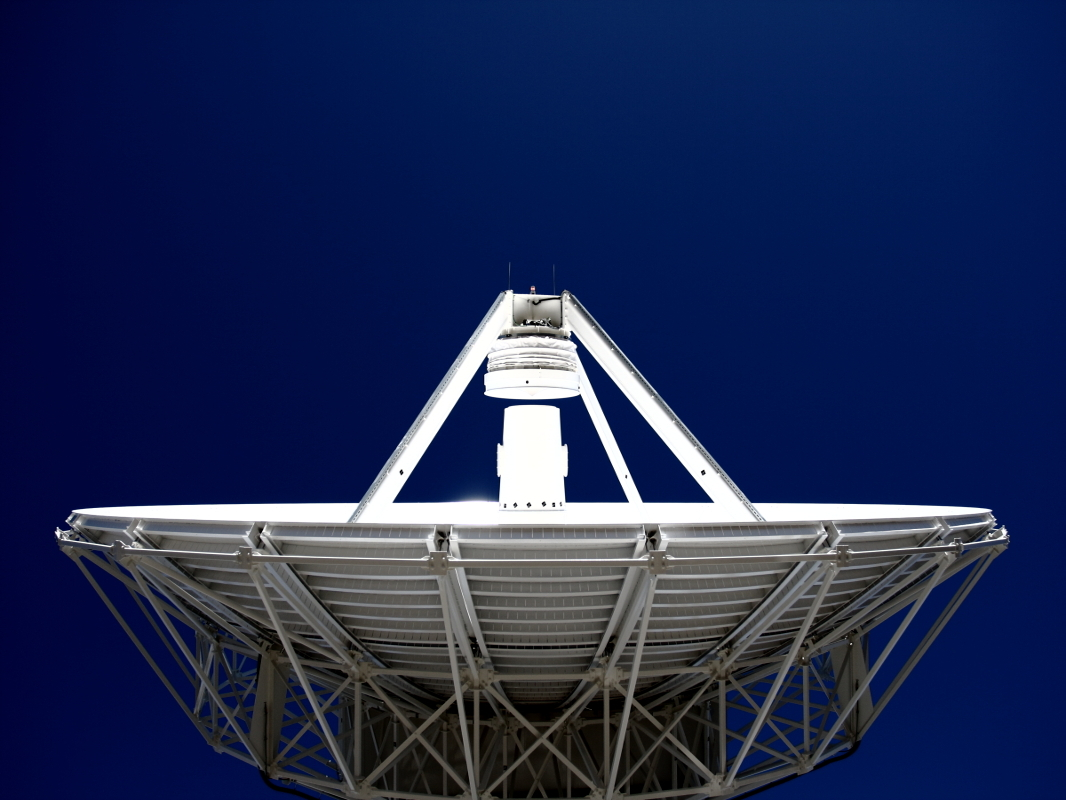
\includegraphics[height=\paperheight]{figure/nyal9}
    }
    \frame[plain,t]{\titlepage}
}

\begin{frame}{Background}
  \begin{itemize}
  \item Acquired the software GEOSAT from NDRE (Norwegian Defence Research Establishment) 
  \item Became an associated IVS analysis center in 2010
  \item Attempted to contribute to ITRF2014
  \item Abandoned GEOSAT in 2015
  \item Then \textbf{Where} was conceived 
  \end{itemize}
\end{frame}

\begin{frame}{What is \textbf{Where}?}
\begin{itemize}
  \item A new software for geodetic analysis
  \item Main focus on VLBI, SLR and GNSS
  \item Based on Python 3 and Cython
  \item Works on multiple platforms
  \item Freely available on GitHub
\end{itemize}
\end{frame}

\begin{frame}{Developers}

\begin{columns}[t]
\vspace{10px}
    \column{0.24\textwidth}
    \begin{center}
      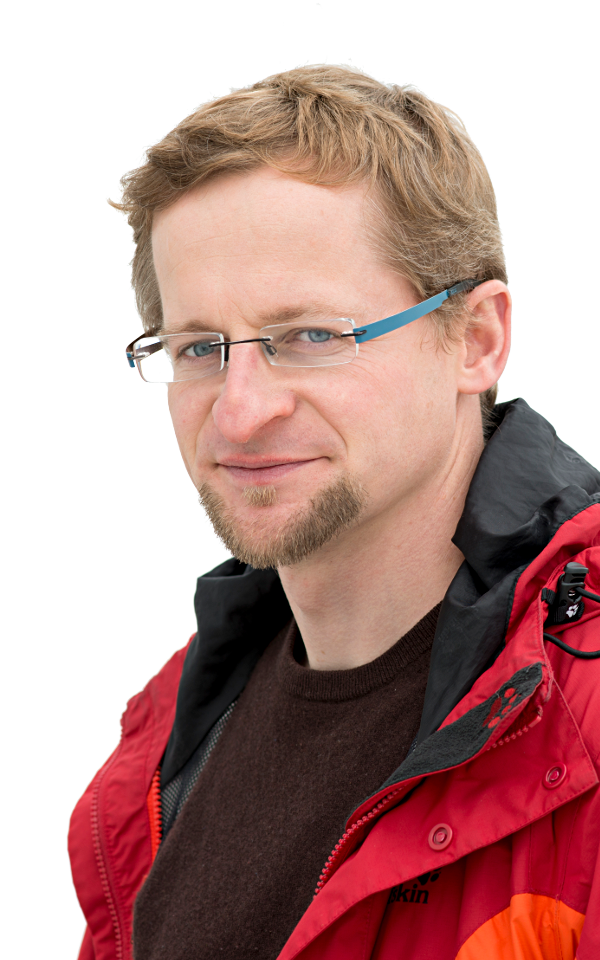
\includegraphics[width=\linewidth]{figure/michael} \\
      Michael D\"ahnn
    \end{center}

    \column{0.24\textwidth}
    \begin{center}
      
\includegraphics[width=\linewidth]{figure/ingrid} \\
      Ingrid Fausk
    \end{center}

    \column{0.24\textwidth}
    \begin{center}
      
\includegraphics[width=\linewidth]{figure/geirarne} \\
      Geir Arne Hjelle
    \end{center}

    \column{0.24\textwidth}
    \begin{center}
      
\includegraphics[width=\linewidth]{figure/annsilje} \\
      Ann-Silje Kirkvik
    \end{center}
  \end{columns}
\end{frame}

\begin{frame}{Motivation}
  \begin{centering}
    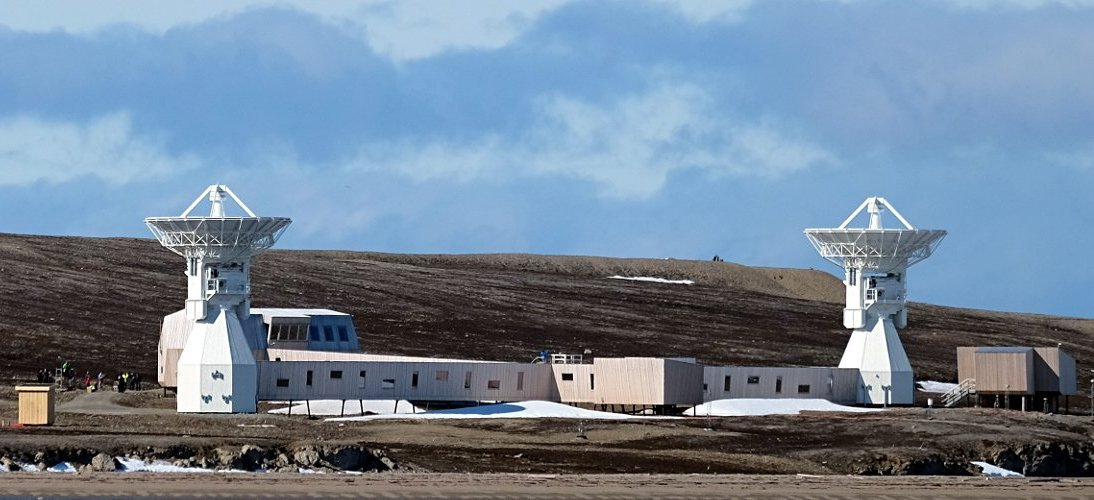
\includegraphics[width=.8\paperwidth]{figure/brandal}
  \end{centering}
\end{frame}

\begin{frame}{Motivation}
  \begin{itemize}
  \item Use our own data
  \item Evaluate station performance
  \item Build VLBI and SLR expertise and ensure continuity
  \item Contribute to reference frame realization and determination of Earth orientation parameters
  \end{itemize}
\end{frame}


\begin{frame}{International collaboration}
\begin{itemize}
  \item NMA has a cooperation agreement with IGN of Spain and the Yebes observatory
  \item IGN provides the receivers and technical assistance for the VLBI antennas in Ny-{\AA}lesund
  \item NMA provides analysis software and support for the new analysis group at IGN 
\end{itemize}
\end{frame}


\begin{frame}{Architecture}
  \begin{columns}
    \begin{column}[c]{0.44\textwidth}
      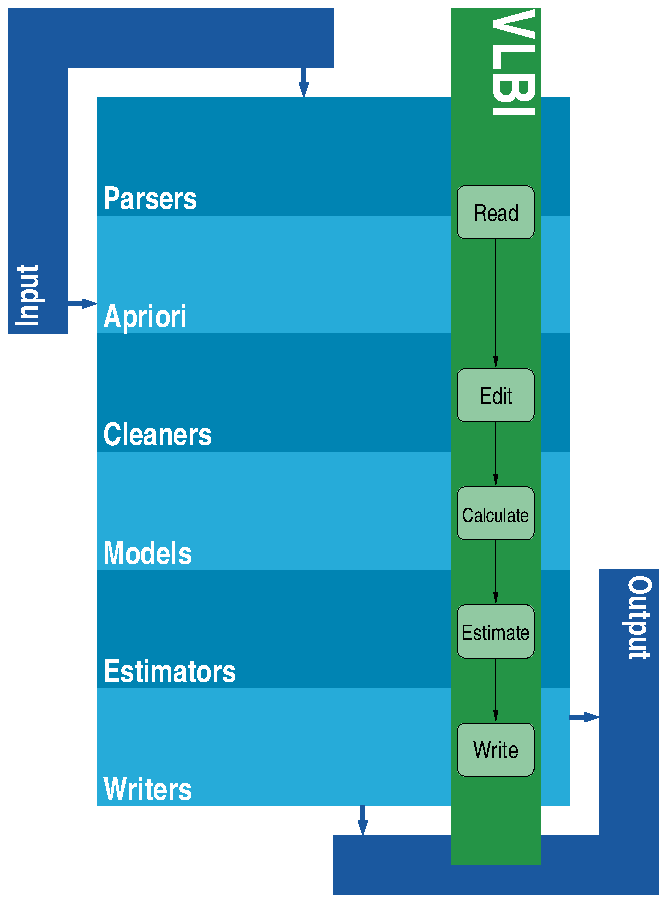
\includegraphics[width=\textwidth]{figure/code_structure_vlbi}
    \end{column}

    \begin{column}[c]{0.55\textwidth}
      An analysis in Where is a pipeline consisting of stages:

      \begin{small}
      \begin{itemize}
      \item Data are stored at each stage
      \item Different analyses use different pipelines
      \item Different pipelines can have different stages
      \item Different pipelines may use the same information sources or modules
      \end{itemize}
      \end{small}
    \end{column}
  \end{columns}
\end{frame}

\begin{frame}[fragile]{How to use \textbf{Where}}
To run an analysis with default configuration:
\begin{shaded*}\texttt{where 2015 8 4 --vlbi --session=XA}\end{shaded*}
To inspect the output graphically: 
\begin{shaded*}\texttt{there 2015 8 4 --vlbi --session=XA}\end{shaded*}
\end{frame}

\begin{frame}{\textbf{There}}
\begin{centering}
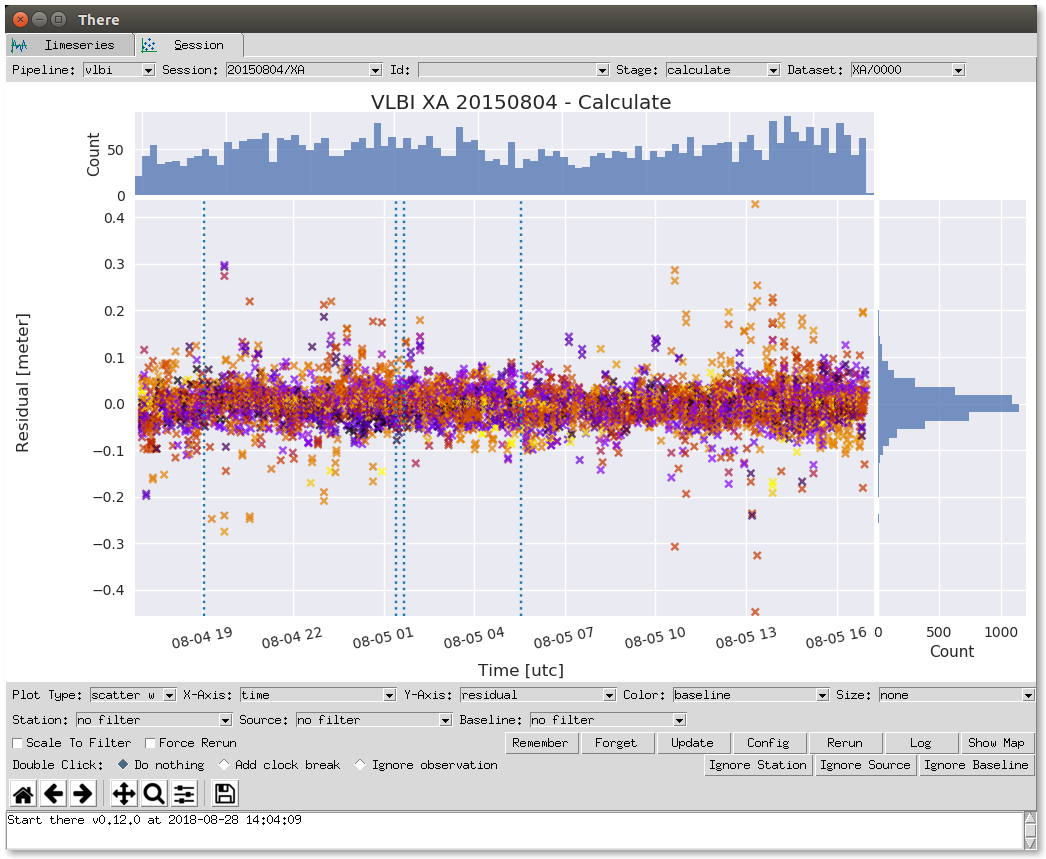
\includegraphics[height=0.8\textheight]{figure/there_residuals}
\end{centering}
\end{frame}


\begin{frame}{More information}
\begin{centering}
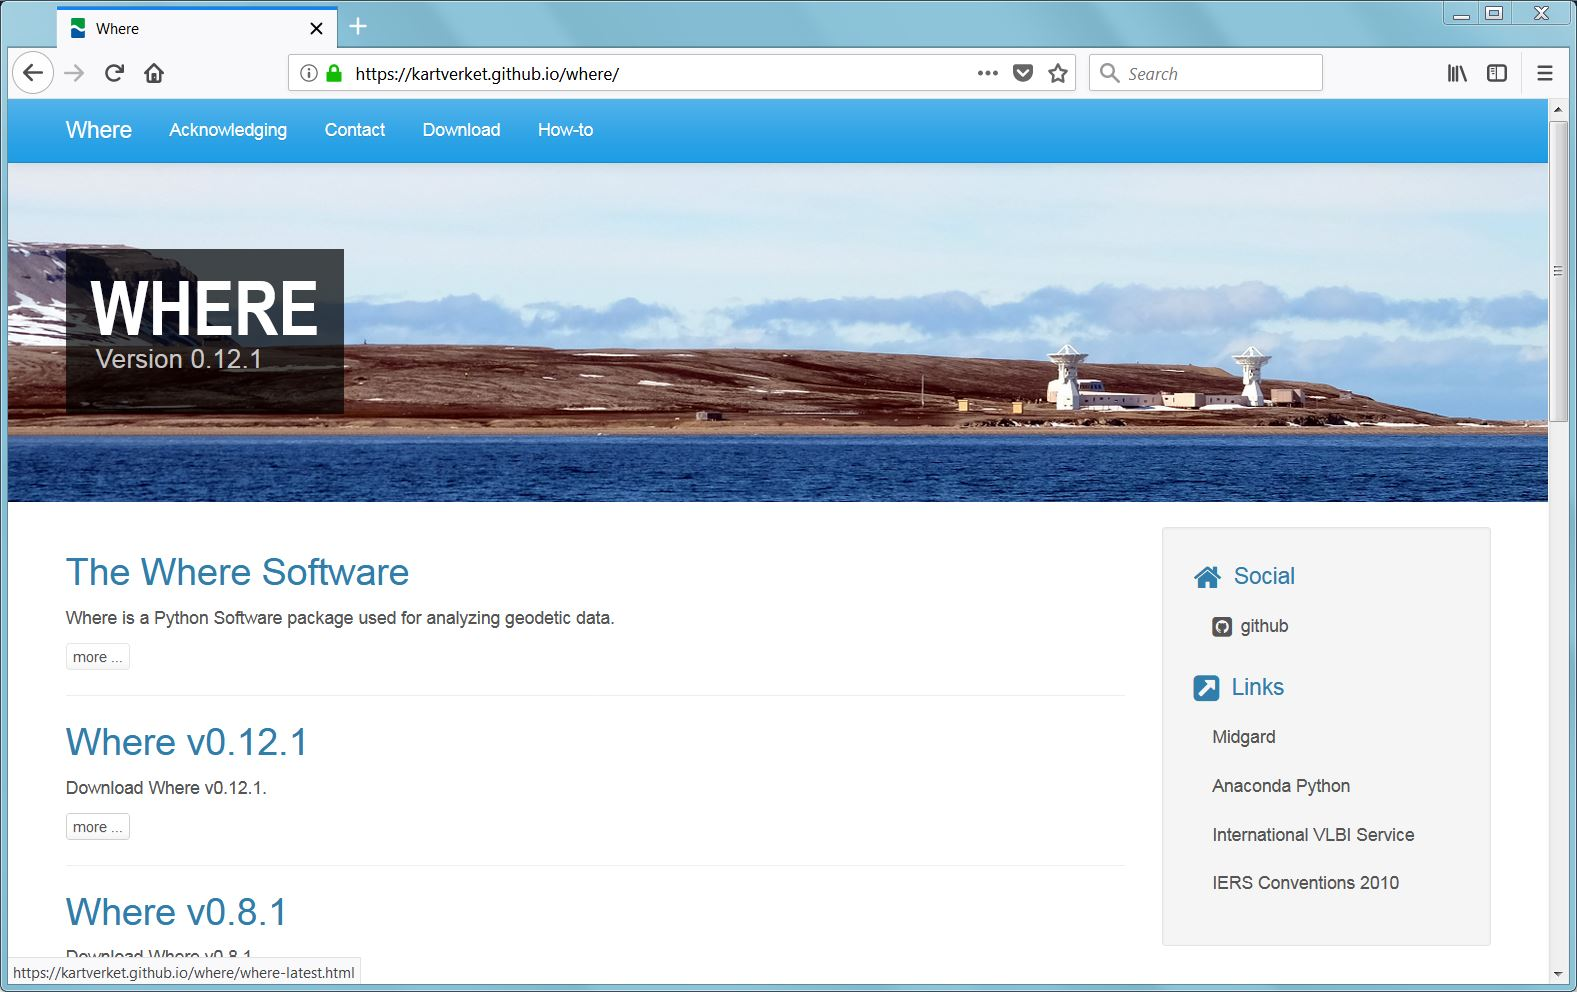
\includegraphics[width=0.95\linewidth]{figure/screenshot_github}
\end{centering}
\end{frame}

\begin{frame}{kartverket.github.io/where}
Current version is 0.12.1
  \begin{itemize}
  \item MIT Open Source License: Permissive, use Where as you want
  \item But please acknowledge us if you use Where
  \item Get in touch if you are interested in Where
  \item This release only includes the VLBI pipeline
  \item Release of version 1.0 is planned this year 
  \end{itemize}
\end{frame}


\begin{frame}{VASCC 2015}
 The VLBI Analysis Software Comparison Campaign
\begin{small}
  \begin{itemize}
  \item Compare computed theoretical delay model of different software packages
  \item 11 participants and 6 solutions found to be consistent within 1~mm
  \item NMA participated in VASCC with GEOSAT
  \item GEOSAT was not consistent, but VieVs and c5++ were
  \item When \textbf{Where} matured the VASCC data was analyzed and compared to the VieVS and c5++ solution
  \end{itemize}
  \end{small}
\end{frame}


\begin{frame}{\textbf{Where} vs VieVS and c5++}
  \begin{itemize}
    \item 2 networks
    \item 1 minute sampling interval
    \item 16 days
  \end{itemize}
  RMS (in mm) of difference between solutions:

\vspace{1em}

  \begin{tabularx}{\columnwidth}{lrCCC}
  & & \multicolumn{3}{c}{Northern}   \\ \cline{3-5}
  &         & \textbf{Where}  & \textbf{c5++}   & \textbf{VieVS}  \\
  \multirow{3}{*}{\rotatebox[origin=c]{90}{Southern}}
    & \multicolumn{1}{|l}{\textbf{Where}} & $\diamond$ &     $0.49$ &     $0.44$ \\
    & \multicolumn{1}{|l}{\textbf{c5++}}  &     $0.18$ & $\diamond$ &     $0.21$ \\
    & \multicolumn{1}{|l}{\textbf{VieVS}} &     $0.43$ &     $0.39$ & $\diamond$ \\
  \end{tabularx}

\end{frame}

\begin{frame}{IVS analysis center}
NMA aims to become a full analysis center by regulary processing R1 and R4 sessions.

\begin{itemize}
  \item When GEOSAT was abandoned this goal was put on hold
  \item With \textbf{Where} maturing the work was resumed
  \item Submitted 5 solutions to the IVS combination center so far
  \item Based on feedback each solution improved upon the previous
  \item Currently awaiting feedback on the 5th solution
\end{itemize}
\end{frame}

\begin{frame}{Station coordinates}
  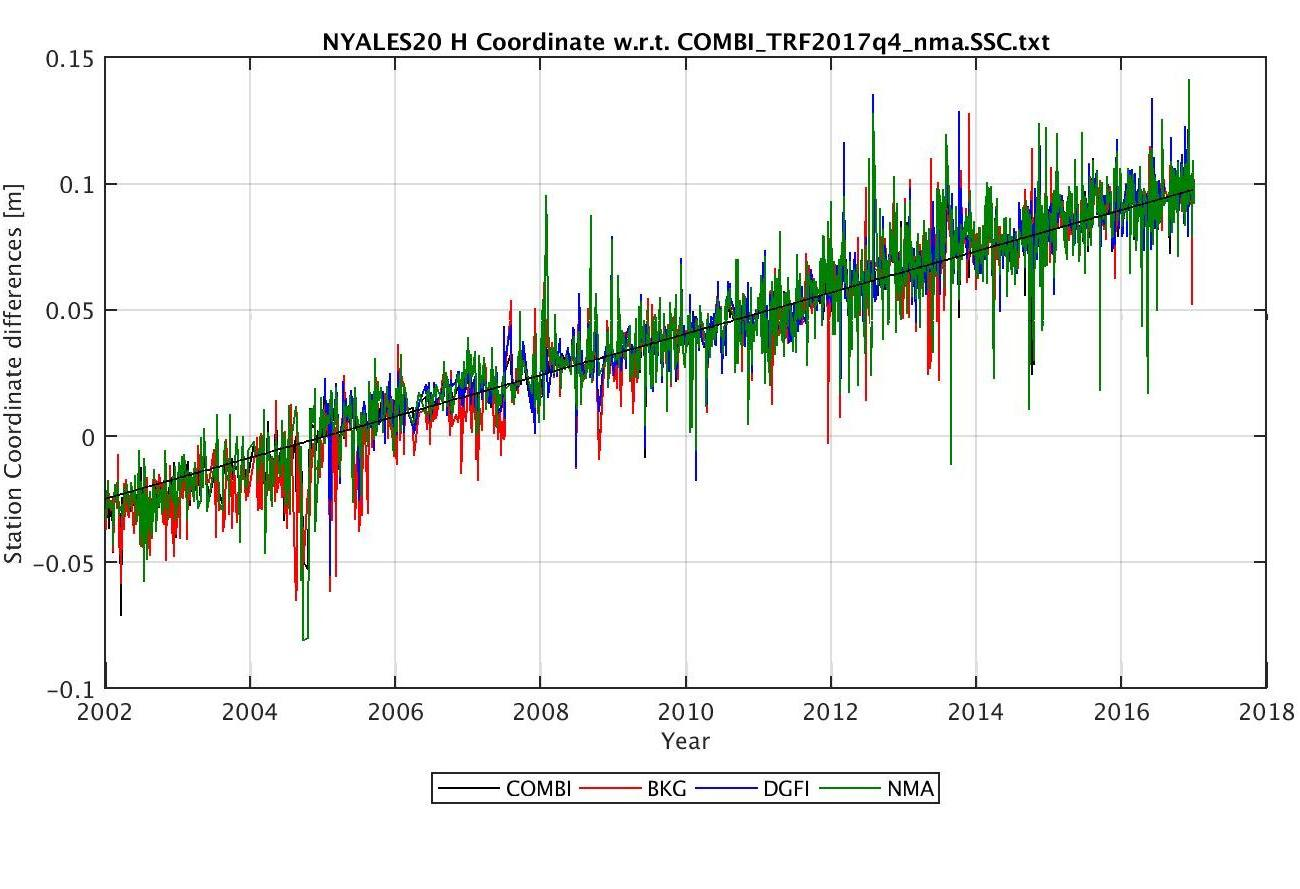
\includegraphics[width=\linewidth]{figure/NYALES20-H_diff-trf}
\end{frame}

\begin{frame}{UT1 - UTC}
  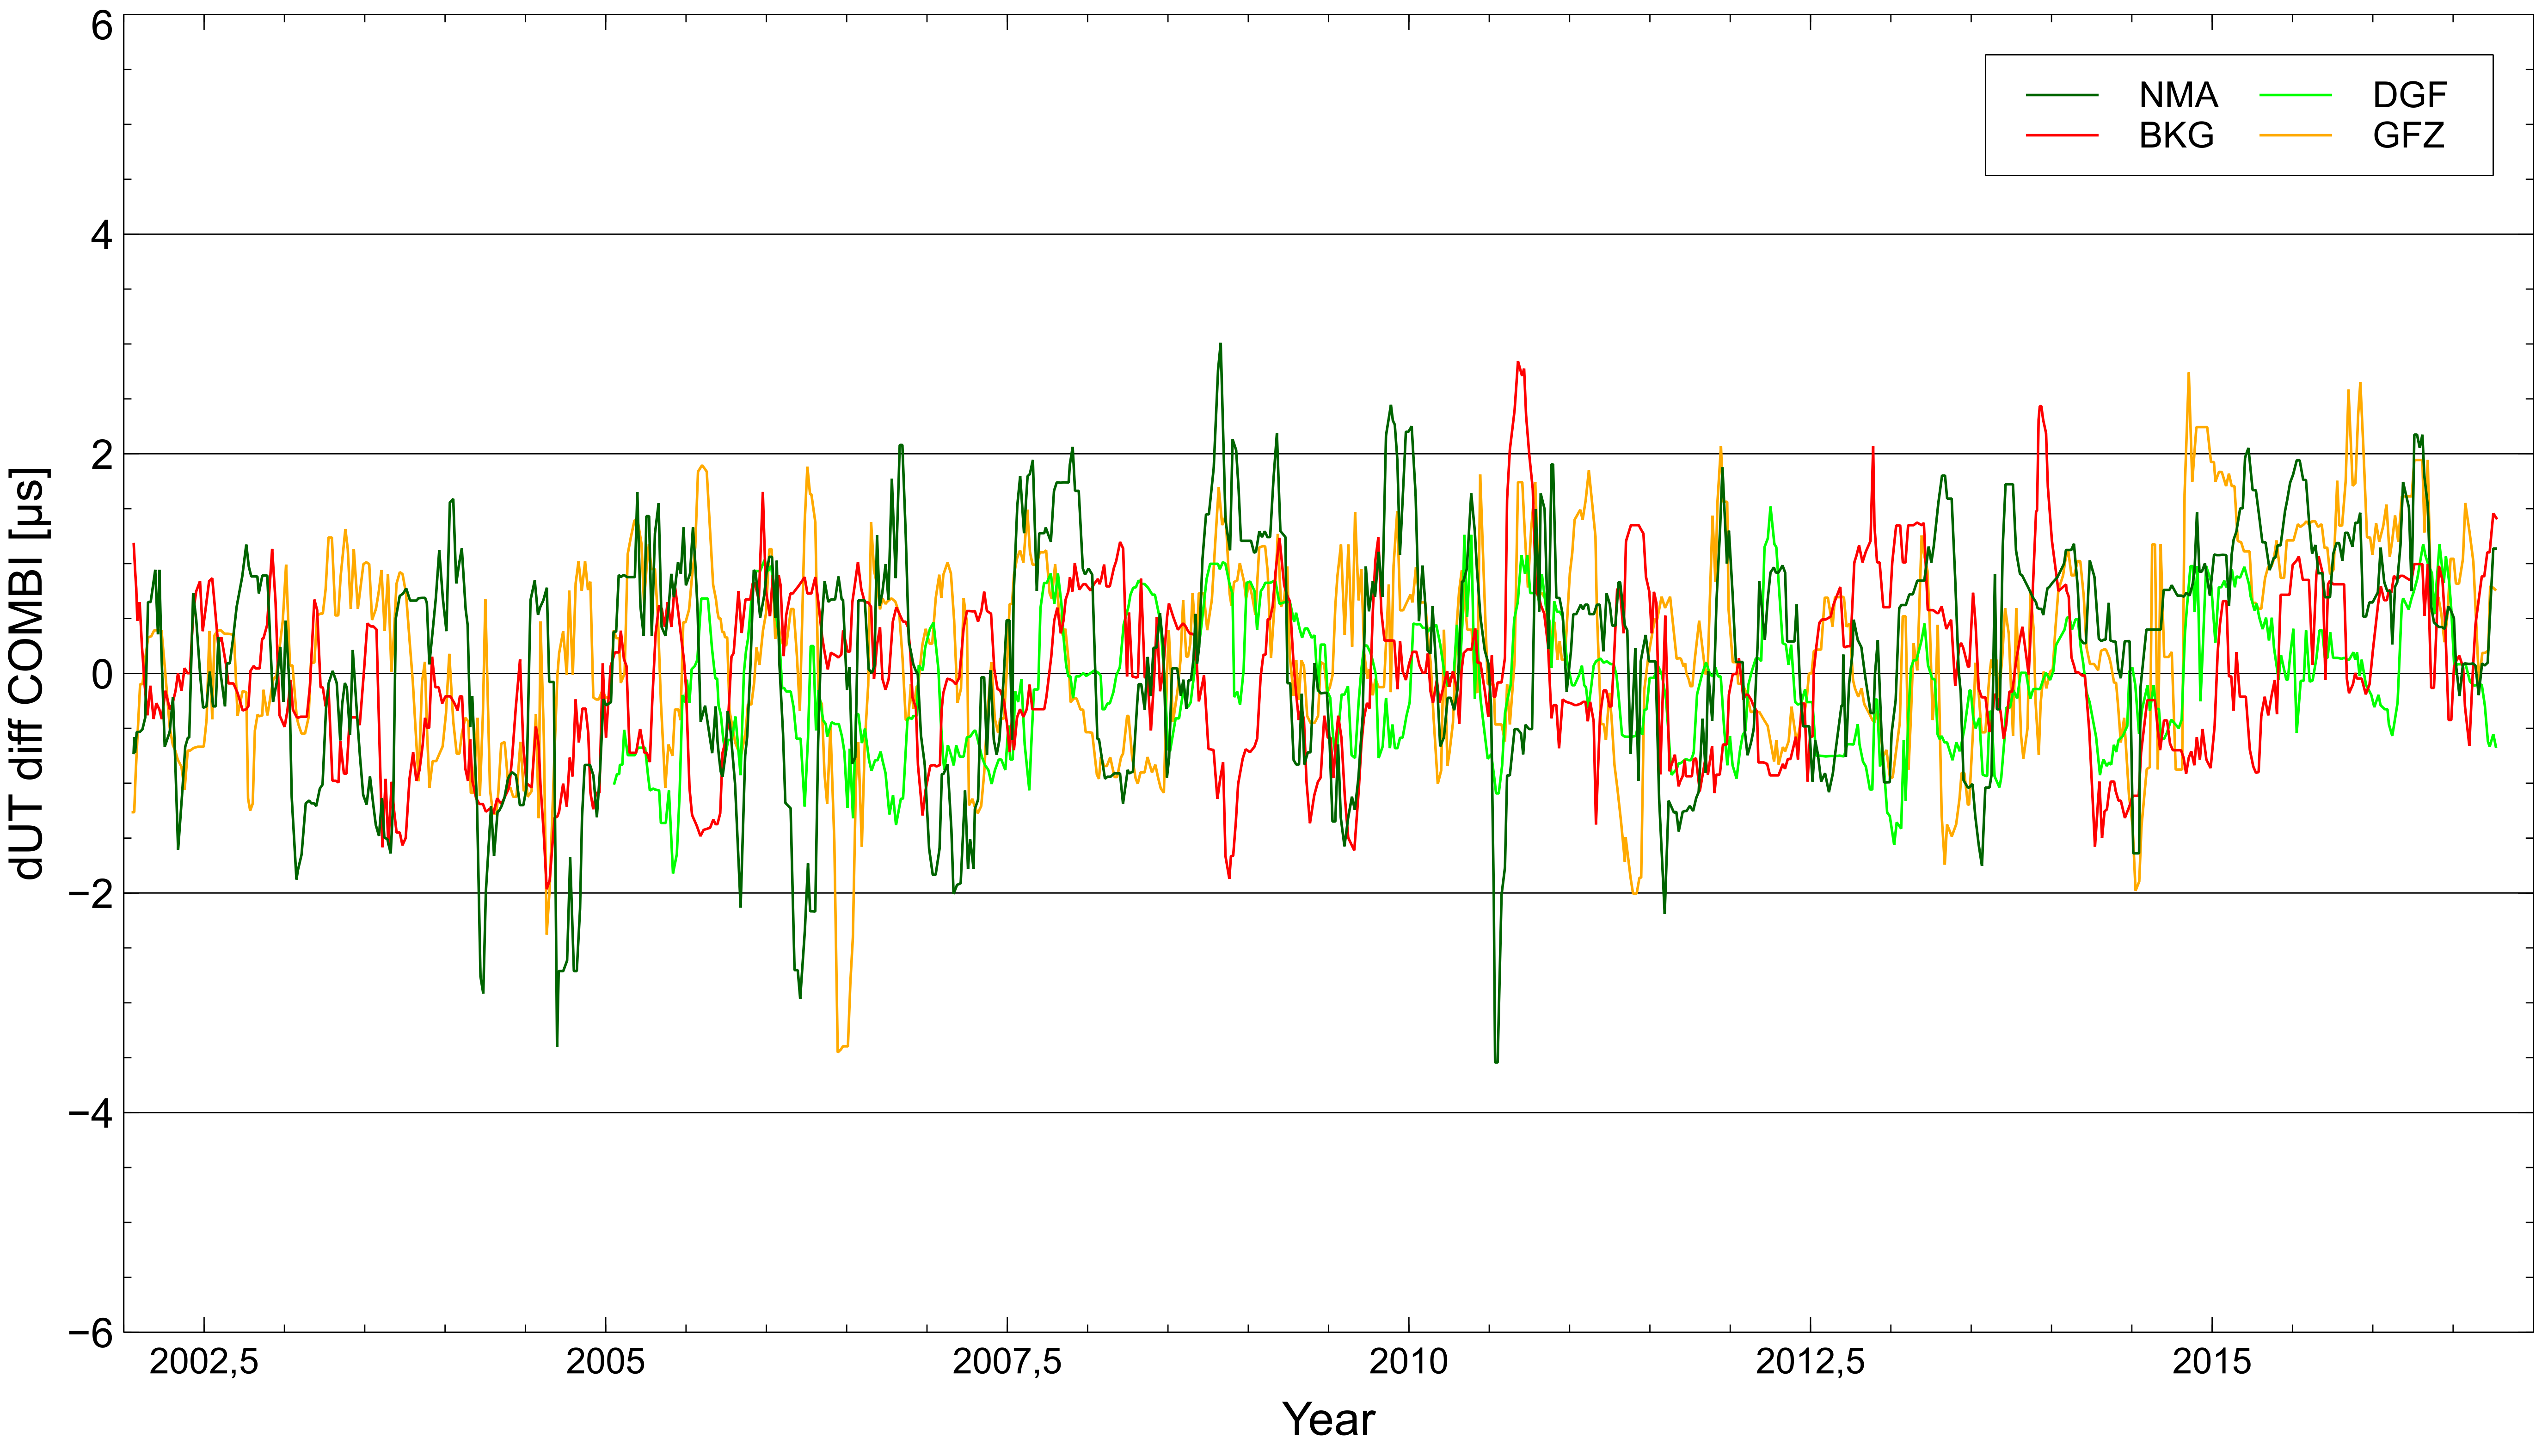
\includegraphics[width=\linewidth]{figure/dut_nma_diff_combi}
\end{frame}

\begin{frame}{LOD}
  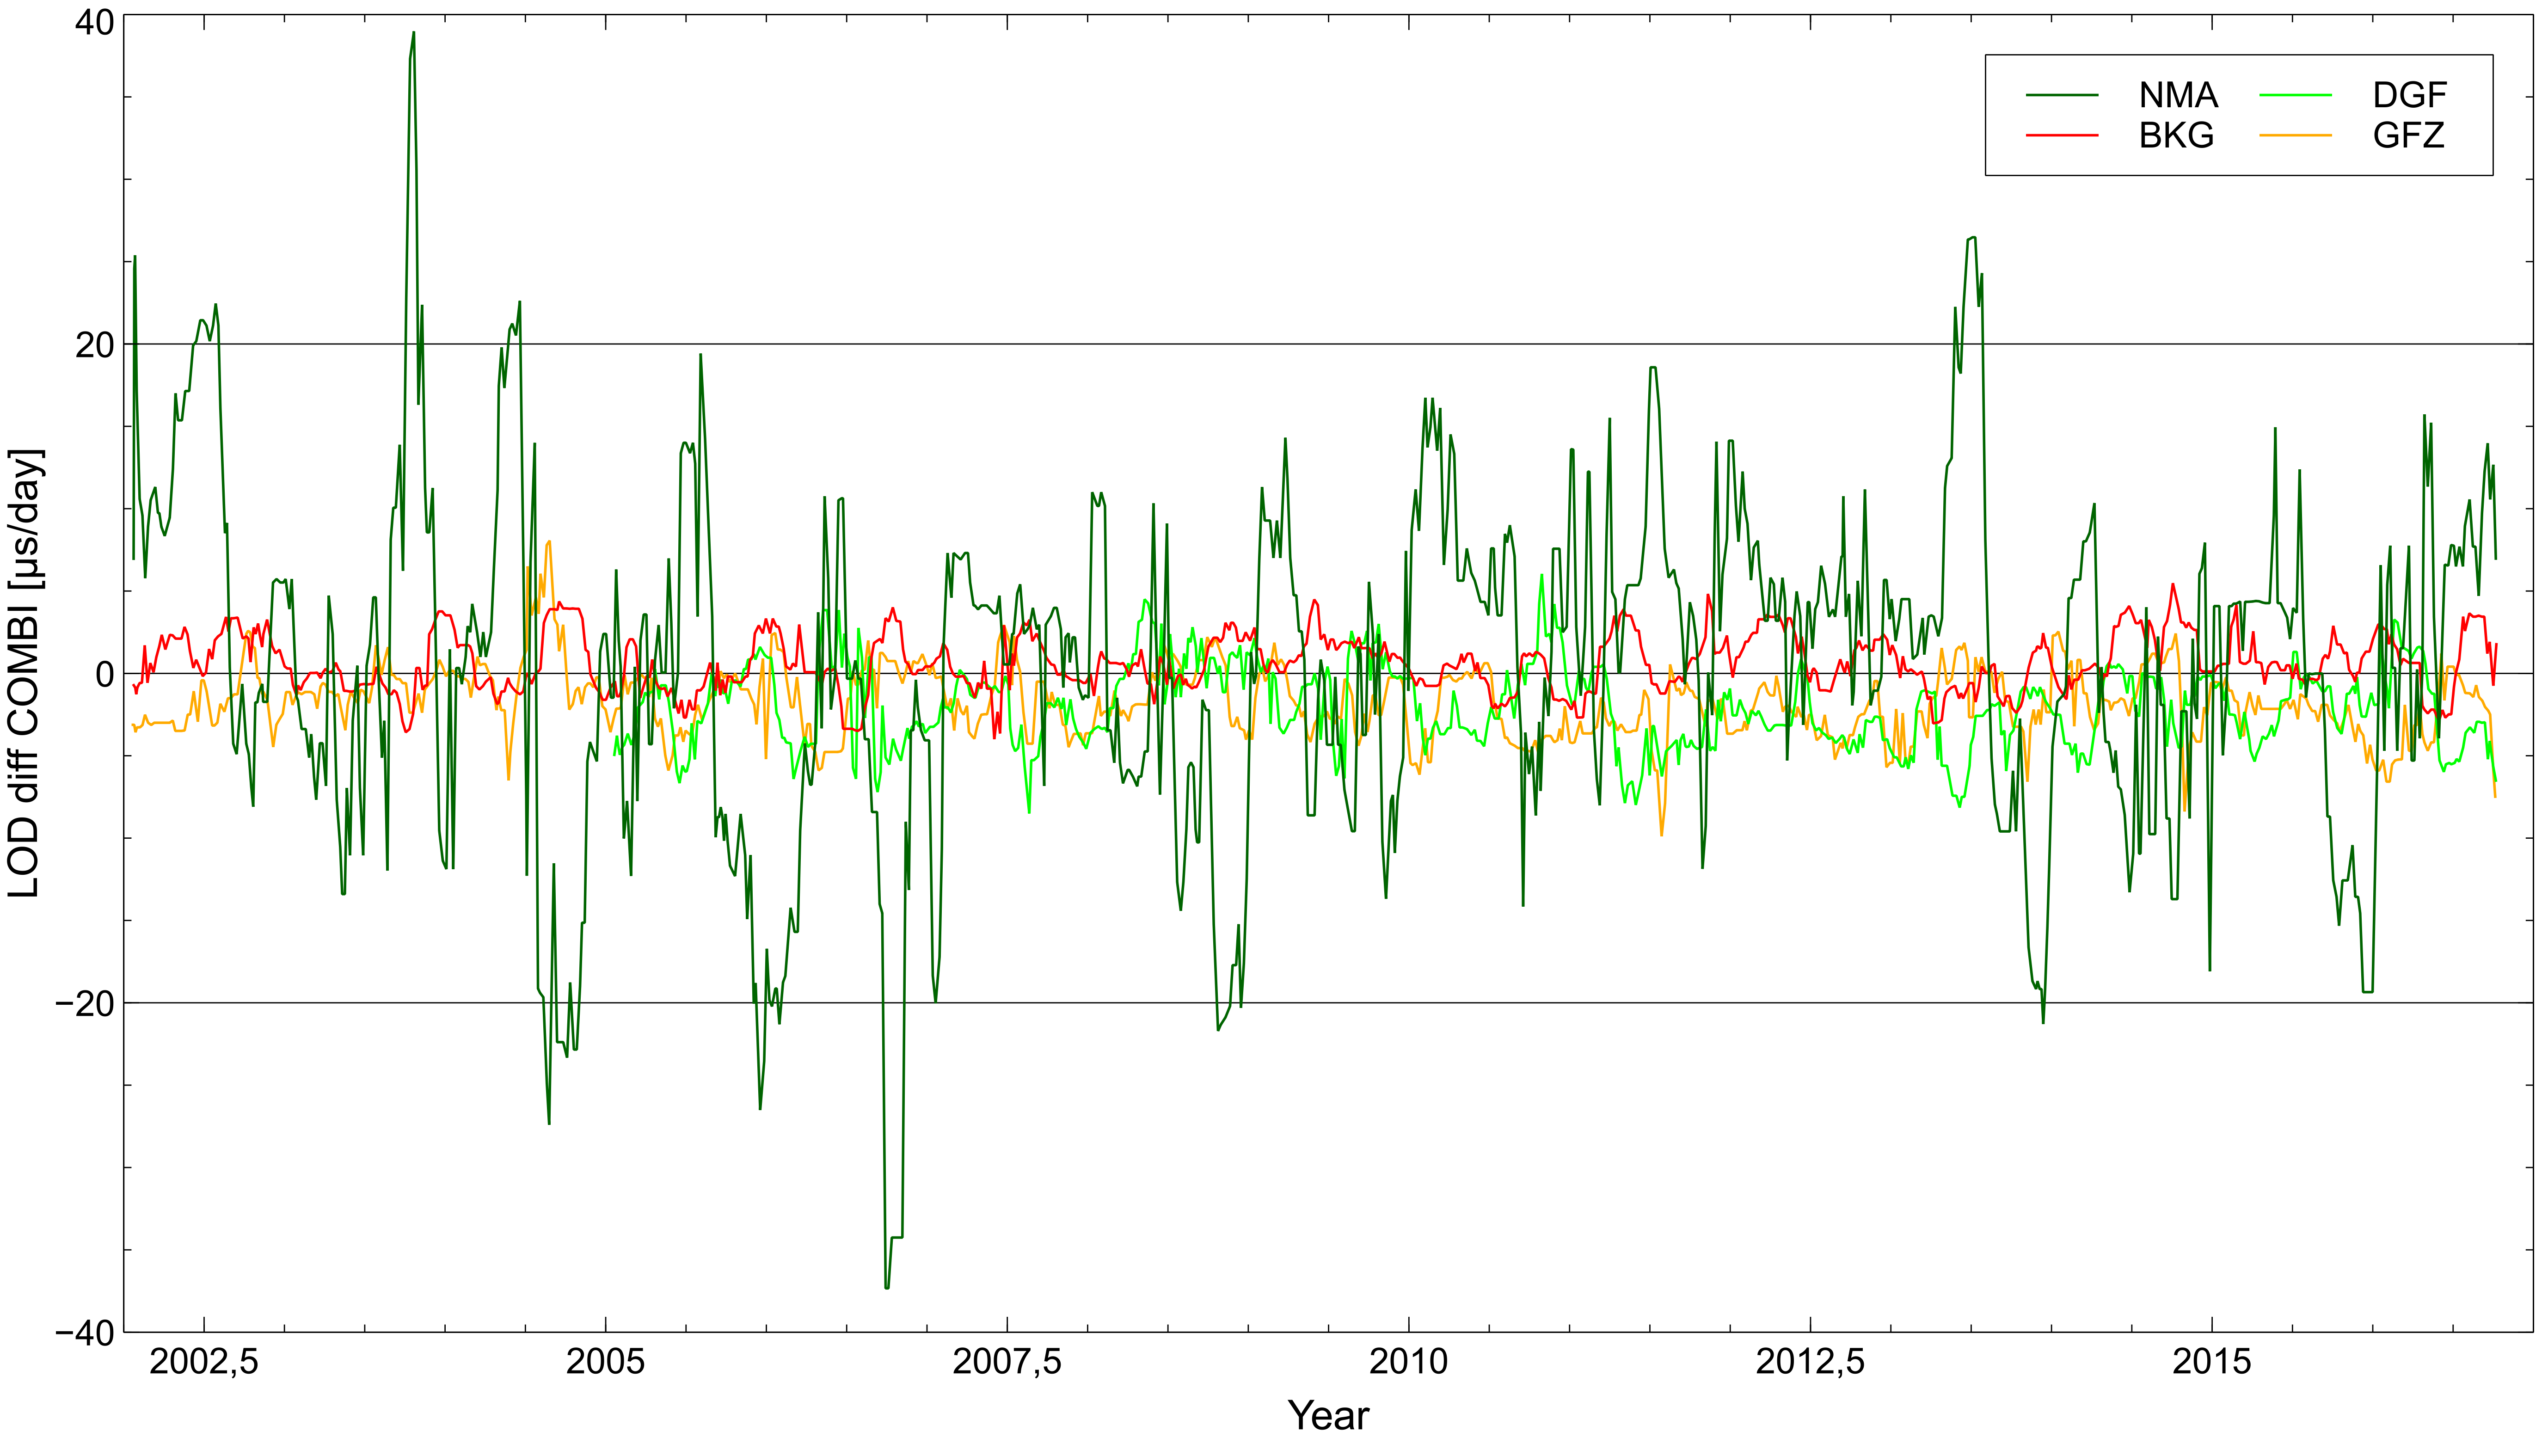
\includegraphics[width=\linewidth]{figure/lod_nma_diff_combi}
\end{frame}


\begin{frame}{Summary}

  \begin{centering}
    Some of the things we are working on at the moment:
  \end{centering}

  \begin{itemize}
  \item Finalize version 1.0 of \textbf{Where}
  \item Set up infrastructure for delivering operational analysis
  \item Cooperate with Yebes/IGN
  \end{itemize}
\end{frame}

\begin{frame}{Questions?}
  \large{https://kartverket.github.io/where/}
\end{frame}


\end{document}
